% Capítulo 2
\chapter{Fundamentação Teórica} \label{ch:fundamentacao-teorica}

Este capítulo apresenta conceitos importantes para a compreensão deste trabalho. A seção \ref{sec:arquitetura-software} explora os conceitos de arquitetura de software e atributos de qualidade, incluindo a definição de cenários. A seção \ref{sec:visualizacao-software} discorre sobre os conceitos de visualização de software, além de definições sobre a visualização da evolução de arquitetura de software. Na seção \ref{sec:ferramentas-analise-desempenho}, são explanados os conceitos empregados nas ferramentas de análise de desempenho. Por fim, na seção \ref{sec:consideracoes-cap2} são apresentadas as considerações finais do capítulo.

\section{Arquitetura de Software} \label{sec:arquitetura-software}

O estudo da arquitetura de software é o estudo de como sistemas de software são projetados e construídos. Ela deve ser o coração do projeto e desenvolvimento de um sistema, estando acima dos processos, análises e do desenvolvimento \cite{Taylor2009}.

A arquitetura de software pode ser definida como a estrutura ou estruturas do sistema, que compreendem os elementos de software, as propriedades externamente visíveis desses elementos e as relações entre eles \cite{Bass2007}. Adicionalmente, de acordo com \citeauthor{Taylor2009}, a arquitetura de um software incorpora todas as decisões de projeto tomadas pelos seus arquitetos, que podem afetar muitos dos seus módulos, incluindo sua estrutura e atributos de qualidade.

Antes da implementação do sistema, decisões arquiteturais tais como quais componentes pertencem a arquitetura do software, quais serviços ou propriedades desses componentes serão externamente visíveis e como eles estão relacionados uns com os outros, devem ser tomadas e deveriam permanecer atendidas durante todo o ciclo de vida do sistema. É igualmente importante o fato de  perceber que a arquitetura do software é essencial para o sistema alcançar os requisitos relacionados aos atributos de qualidade \cite{Kazman2001}.

\subsection{Atributos de Qualidade} \label{subsec:atributos-qualidade}

A medida que o domínio de um software evolui, assim como os seus requisitos, a arquitetura do software precisa ser reavaliada de modo que ainda reflita um sistema moderno que se encaixa no domínio evoluído. Uma arquitetura não é regida apenas por requisitos funcionais, mas em grande parte por atributos de qualidade. Desse modo, criar uma arquitetura apropriada não é uma tarefa trivial \cite{Svahnberg2002}.

A qualidade não pode ser adicionada ao sistema de maneira tardia, pelo contrário, deve ser incorporada desde o início \cite{Svahnberg2002}. Portanto, a arquitetura de um software necessita ser reavaliada para verificar a conformidade dos requisitos funcionais e atributos de qualidade.

Os atributos de qualidade que serão analisados em um processo de avaliação dependem do contexto e domínio do sistema. Uma estratégia comum é abordar os atributos de qualidade mais críticos. Alguns desses atributos são definidos adiante \cite{Kazman2001}:
\begin{itemize}
	\item \textit{Desempenho}: trata da capacidade de resposta do sistema, o tempo requerido para responder a eventos ou o número de eventos processados em determinado intervalo de tempo;
	\item \textit{Confiabilidade}: é a habilidade do sistema se manter operante com o passar do tempo. É geralmente medido pelo tempo médio até a falha;
	\item \textit{Segurança}: mede a habilidade do sistema de resistir a tentativas de uso não autorizado e negação de serviço, enquanto continua fornecendo seus serviços a usuários autorizados;
	\item \textit{Portabilidade}: é a capacidade do sistema de executar em diversos ambientes computacionais.
\end{itemize}

Embora existam outros atributos de qualidade, o atributo de interesse deste trabalho é o desempenho, em termos de tempo de execução. O desempenho será destacado como uma das principais informações mostradas nas visualizações descritas posteriormente.

\subsection{Avaliação Baseada em Cenários} \label{subsec:avaliacao-baseada-cenarios}

Algumas abordagens de avaliação arquitetural foram propostas para lidar com questões relacionadas com a qualidade em arquiteturas de software, dentre elas, a avaliação baseada em cenários é considerada bastante madura \cite{Babar2004}. O propósito dessa avaliação é exercitar os cenários com a finalidade de determinar se a arquitetura é adequada para um conjunto de atributos de qualidade.

Um cenário é definido pela interação entre os \textit{stakeholders} e o sistema. Eles são particularmente úteis para ajudar os arquitetos a entender como os atributos de qualidade podem ser abordados. Os \textit{stakeholders} podem ter diferentes perspectivas dos cenários. Por exemplo, um usuário pode imaginar um cenário como uma tarefa que ele precisa fazer no sistema. Por outro lado, um desenvolvedor, que irá implementar o cenário, pode focar em uma visão arquitetural e usar a arquitetura do software para guiar o processo de desenvolvimento \cite{Pinto2015}.

Nesse contexto, os cenários se tornam especialmente úteis quando os programadores e arquitetos precisam obter uma melhor compreensão sobre os atributos de qualidade, uma vez que especificam todos os tipos de operações que o sistema terá que executar para atender a determinadas funcionalidades. Assim, uma análise detalhada do modo como essas operações serão implementadas, executadas ou até mesmo se elas podem falhar ou não, ajuda os avaliadores a extrair informações importantes sobre os atributos de qualidade, por exemplo, o desempenho.

\section{Visualização de Software} \label{sec:visualizacao-software}

A área visualização de software é parte da visualização da informação e pode ser definida, de maneira ampla, como a visualização de artefatos relacionados ao software e seu processo de desenvolvimento. Adicionalmente ao código-fonte do programa, esses artefatos incluem documentação de requisitos e projeto, mudanças no código-fonte e relatório de \textit{bugs}, por exemplo \cite{Diehl2007}. Ainda de acordo com \citeauthor{Diehl2007}, a visualização de software é a arte e ciência de gerar representações visuais de vários aspectos de um software e de seu processo de desenvolvimento. O objetivo principal é ajudar a compreender sistemas de software e aumentar a produtividade do processo de desenvolvimento.

Essas representações são necessárias para que os analistas, arquitetos e desenvolvedores examinem os sistemas de software devido à sua natureza complexa, abstrata e difícil de observar \cite{Petre2006}. Tais dificuldades são ainda piores em sistemas de grande escala.

Existem três tipos de aspectos do software que a visualização pode abordar \cite{Diehl2007}:
\begin{enumerate}[(i)]
	\item \textit{Estático}: neste tipo, a visualização do software apresenta o software como ele é codificado, lidando com informações que são válidas para todas as suas possíveis execuções. A estrutura do software em vários níveis de abstração pode ser obtida através desse aspecto, incluindo sua arquitetura;
	\item \textit{Dinâmico}: provê informações sobre uma execução particular do sistema e ajuda a entender o seu comportamento. Pode exibir quais instruções são executadas e como o estado do programa se altera. Exemplos: visualização dinâmica da arquitetura, algoritmos animados e depuração e testes visuais;
	\item \textit{Evolução}: adiciona a variável tempo a visualização dos aspectos estáticos ou dinâmicos do software.
\end{enumerate}

Com relação ao que os usuários visualizam, Gómez Henriquez \cite{Gomez-Henriquez2001a} menciona que a visualização de software é principalmente usada para: (i) exibição do comportamento do programa, normalmente para fins pedagógicos; (ii) depuração lógica; e (iii) depuração de desempenho. Entretanto, a lista pode ser estendida para: atividades de desenvolvimento, depuração, testes, manutenção e detecção de falhas, reengenharia, engenharia reversa, gerenciamento de processo de desenvolvimento e marketing \cite{Maletic2002}. \citeauthor{Diehl2007} sumariza a lista em apenas seis itens: projeto, implementação, testes, depuração, análise e manutenção.

\subsection{Visualização de Arquitetura de Software} \label{subsec:visualizacao-arquitetura-software}

Um dos mais importantes tópicos na área de visualização de software é a visualização da arquitetura do software \cite{Ghanam2008}\cite{Denford2002}\cite{Gallagher2005}\cite{Gallagher2008}. Geralmente, os sistemas orientados a objetos são estruturados de maneira hierárquica, com pacotes contendo subpacotes, recursivamente, e com classes estruturadas por métodos e atributos. Visualizar a arquitetura consiste em observar a hierarquia e os relacionamentos entre os componentes do software \cite{Caserta2011}. No entanto, estudos indicam que, além dos módulos do software, com suas estruturas, relacionamentos e métricas, existe um interesse crescente em visualizar a evolução desses módulos \cite{Ambros2007}.

As representações visuais mais comuns para visualizar a estrutura hierárquica da arquitetura de um software é uma estrutura em árvore \cite{Khan2012}. Exemplos de outras formas de se representar a arquitetura são o \textit{Treemap} retangular \cite{Johnson1991} e circular \cite{Wang:2006:VLH:1124772.1124851} e o \textit{Icicle Plot} \cite{Barlow2001}. Já para a visualização dos relacionamentos, podem ser mencionados: \textit{Dependency Structure Matrix} \cite{Holten2006}, \textit{DA4Java} \cite{Pinzger2008}, \textit{EvoSpaces} \cite{Alam2007} e \textit{Clustered Graph Layout} \cite{Balzer2007}. Para a visualização das métricas de um software, são exemplos as soluções: \textit{Metric View} \cite{Termeer2005}, \textit{Areas of Interest} \cite{Byelas2009} e \textit{CodeCrawler} \cite{Lanza2005}.

\begin{figure}[htb]
	\centering
  	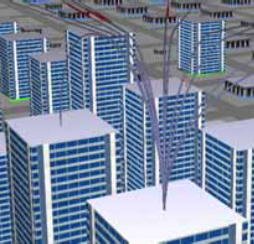
\includegraphics[scale=0.75]{Imagens/evospaces.png}
  	\textsf{\caption[EvoSpaces.]{EvoSpaces \cite{Alam2007}.\label{fig:evospaces}}}
\end{figure}

O EvoSpaces \cite{Alam2007}, mostrado na figura \ref{fig:evospaces}, é uma ferramenta que provê a visualização da arquitetura do software em um ambiente virtual. Aproveita o fato de que os sistemas são, muitas vezes, estruturados hierarquicamente para sugerir o uso de uma metáfora de cidades. As entidades, junto com suas relações, são representadas como glifos residenciais (casa, apartamento, escritório, etc), ao passo que as métricas dessas entidades são exibidas como posições e escalas visuais (tamanho, valor da cor, etc). A ferramenta possui diferentes modos de interação, como \textit{zoom} e capacidades de navegação.

\begin{figure}[htb]
	\centering
  	\frame{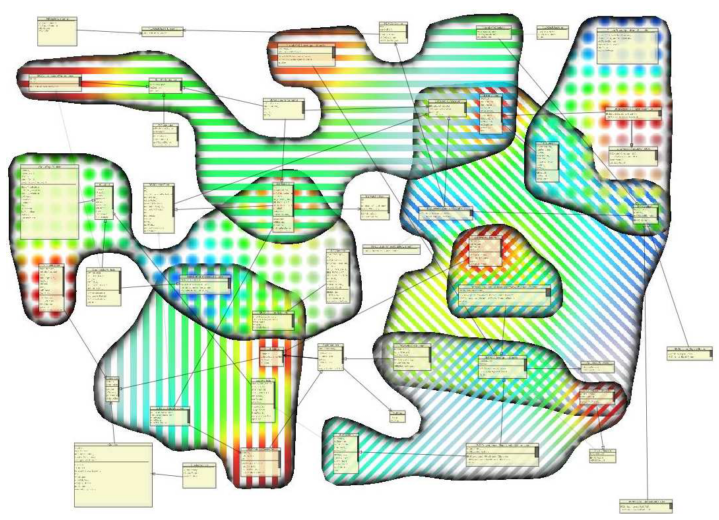
\includegraphics[scale=0.30]{Imagens/areas_of_interest.png}}
  	\textsf{\caption[Areas of Interest.]{Areas of Interest \cite{Byelas2009}.\label{fig:areas-of-interest}}}
\end{figure}

O Areas of Interest \cite{Byelas2009}, mostrado na figura \ref{fig:areas-of-interest}, é uma técnica que consiste em aplicar um algoritmo que agrupa entidades de software com propriedades comuns, as engloba com um contorno e adiciona cores para descrever métricas de software. Para distinguir áreas de sobreposição, cada área tem uma textura diferente, como linhas horizontais, verticais, diagonais e círculos. Além disso, técnicas de sombreamento e transparência são usadas para melhorar a distinção entre várias áreas.

\subsection{Visualização da Evolução da Arquitetura de Software} \label{subsec:visualizacao-evolucao-arquitetura-software}

A evolução de um software tem sido destacada como um dos tópicos mais importantes na engenharia de software \cite{Novais2013}. Trata-se de uma tarefa complexa por gerar grande quantidade de dados e lidar com isso é complicada: estima-se que 60\% do esforço na etapa de manutenção é para entender o software \cite{Corbi1989}. A visualização de software visa ajudar os \textit{stakeholders} a melhorar a compreensão do software, no entanto, elaborar metáforas visuais que representem efetivamente a dimensão tempo com todas as informações relacionadas a evolução do software é uma tarefa difícil \cite{Magnavita2015}.

No contexto da visualização da evolução da arquitetura de um software, um dos grandes desafios, além da quantidade de dados provenientes da evolução, é o crescente tamanho e complexidade do software. Apesar da dificuldade, é importante prover visualizações gerais da arquitetura, dos relacionamentos entre os módulos e das métricas, para cada versão \cite{Khan2012}.

\begin{figure}[htb]
	\centering
  	\frame{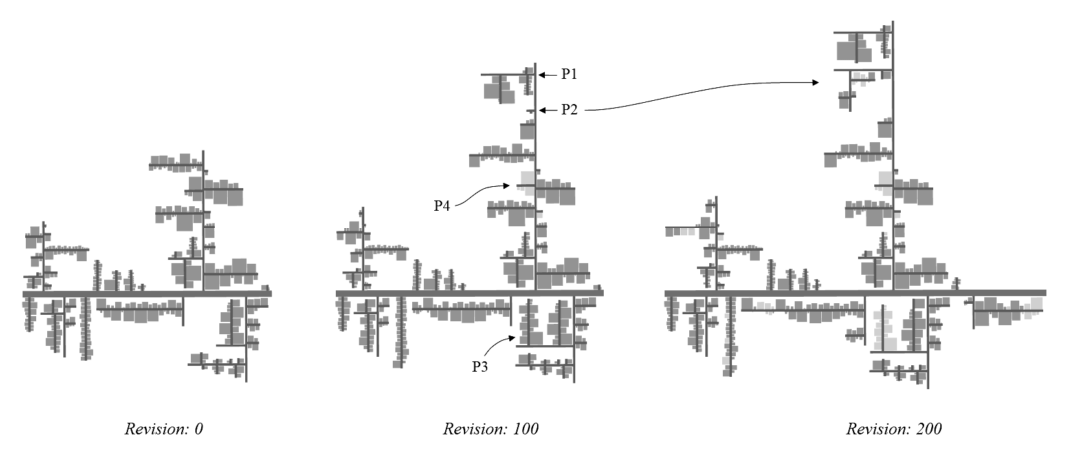
\includegraphics[scale=0.40]{Imagens/crococosmos.png}}
  	\textsf{\caption[CrocoCosmos.]{CrocoCosmos \cite{Steinbruckner2010b}.\label{fig:crococosmos}}}
\end{figure}

O \textit{CrocoCosmos} \cite{Steinbruckner2010b} é um exemplo de ferramenta que utiliza uma metáfora de cidades para representar a evolução estrutural da arquitetura de um software, onde ruas representam pacotes e construções refletem as classes Java. A sequência de representações visuais objetiva destacar as mudanças básicas na estrutura do software, como elementos que foram adicionados, removidos ou movidos dentro da hierarquia. A figura \ref{fig:crococosmos} mostra essa ferramenta. O \textit{Code Flows} \cite{Telea2008} e o \textit{Successive Inheritance Graphs} \cite{Collberg2003} são outros exemplos de visualizações de evolução estrutural de arquitetura de software.

Outra forma de se exibir a evolução de um software é através das suas métricas. Elas encapsulam, sumarizam e provêem informações de qualidade sobre o código-fonte \cite{Langelier2008}. As métricas são essenciais para o entendimento contínuo e para a análise da qualidade do sistema durante todas as fases do seu ciclo de vida \cite{Khan2012}.

O \textit{CodeCity} \cite{Wettel2007} é uma visualização interativa em 3D que avalia a evolução estrutural de sistemas de software e as apresenta utilizando uma metáfora de cidades. As métricas são exibidas através de propriedades visuais dos artefatos da cidade: as propriedades das classes, como o número de métodos e de atributos, são mapeadas como a altura e o tamanho da base das construções, respectivamente; a profundidade dos pacotes é representada através da saturação de cores dos distritos. A figura \ref{fig:codecity} exemplifica essa ferramenta.

\begin{figure}[htb]
	\centering
  	\frame{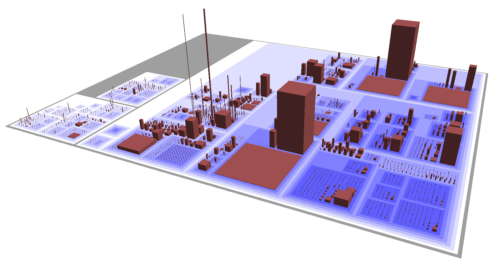
\includegraphics[scale=0.75]{Imagens/codecity.png}}
  	\textsf{\caption[CodeCity.]{Codecity \cite{Wettel2007}.\label{fig:codecity}}}
\end{figure}

Outras soluções que apresentam visualizações da evolução da arquitetura de um software através das métricas são: \textit{The Evolution Matrix} \cite{Lanza2001}, \textit{VERSO} \cite{Langelier2008} e \textit{RelVis} \cite{Pinzger2005}.

\subsection{Estudos Empíricos em Visualização de Software {\color{red} fica ou sai?}} \label{subsec:estudos-empiricos-visualizacao-software}

As visualizações são importantes para ajudar na compreensão de vários aspectos de um software, além de ajudar a aumentar a produtividade do processo de desenvolvimento, lançando mão de metáforas visuais para representar esses aspectos. Entretanto, não significa que toda visualização de software é útil. Para cada técnica em particular, e para cada intenção de uso, é necessário avaliar a sua utilidade \cite{Diehl2007}. O objetivo principal de uma visualização é transmitir informações de forma compreensível, eficaz e fácil de lembrar. \citeauthor{Diehl2007} agrupa as avaliações das visualizações em dois grupos: quantitativa e qualitativa.

Os métodos quantitativos de avaliação medem propriedades da visualização ou propriedades do usuário interagindo com a visualização. Esse tipo de avaliação requer uma análise estatística dos resultados de um experimento controlado \cite{Diehl2007}.

Já o método qualitativo coleta dados sobre a experiência dos usuários com as visualizações, verbalizados em formato de relatórios. Os métodos qualitativos são de extrema importância quando se trata da percepção humana e da interação com uma visualização \cite{McConathy1993}, incluindo o fato de eles exigirem menos pessoas para o teste e cobrirem mais aspectos da visualização avaliada.

\citeauthor{komlodi2004information}, em sua pesquisa com cerca de 50 estudos de usuários de sistemas de visualização de informação, encontrou quatro áreas de avaliação:
\begin{enumerate}[(i)]
	\item \textit{Experimentos controlados comparando elementos de design}: esses estudos podem comparar elementos específicos;
	\item \textit{Avaliação de usabilidade de uma ferramenta}: esses estudos podem fornecer \textit{feedback} sobre problemas encontrados pelos usuários com uma ferramenta e mostrar como os \textit{designers} podem refinar o \textit{design};
	\item \textit{Experimentos controlados comparando duas ou mais ferramentas}: geralmente tentam comparar novas abordagens com o estado da arte;
	\item \textit{Estudos de caso de ferramentas em contextos realistas}: a vantagem dos estudos de caso é que eles relatam os usuários em seu ambiente natural fazendo tarefas reais, demonstrando viabilidade e utilidade no contexto. A desvantagem é que eles são demorados para conduzir e os resultados podem não ser replicáveis e generalizáveis.
\end{enumerate}

\citeauthor{Seriai2014} realizou um estudo de mapeamento sistemático de métodos de validação em visualização de software. Os autores definiram seis propriedades de classificação desses métodos:
\begin{enumerate}[(i)]
	\item \textit{Tipo de Investigação}: determina qual o tipo de estudo empírico foi usado: experimento, estudo de caso ou questionário;
	\item \textit{Tarefas}: especifica a natureza das tarefas envolvidas na avaliação. Elas são específicas quando o participante tem que resolver um problema específico, ou exploratórias quando o participante não tem uma tarefa específica para executar;
	\item \textit{Fonte de Dados}: caracteriza a fonte dos dados da visualização: industrial, open source e/ou dados domésticos;
	\item \textit{Participantes}: determina o perfil dos participantes usados na avaliação, se houver: estudantes, profissionais ou ambos;
	\item \textit{Medidas}: especifica se a avaliação incluiu medidas objetivas, ou seja, sem ser baseadas no julgamento dos participantes. Caso contrário, as medidas poderiam ser subjetivas ou sem medida
	\item \textit{Referência de Comparação}: define se a ferramenta foi comparada a outras ferramentas.
\end{enumerate}

Como resultados, os autores destacam que 78,16\% dos artigos analisados utilizaram o método de estudo de caso, sendo destes, 65\% puramente análise qualitativa. Além disso, 72,5\% envolviam tarefas específicas na avaliação, 77\% dos artigos usaram ferramentas open source, 70,1\% das avaliações foram realizadas sem participantes. Com relação às medidas, 60,9\% dos trabalhos coletaram medidas objetivas. Por fim, 77\% dos artigos não incluíram nenhuma comparação com outras abordagens. Baseado nesses resultados, os autores concluíram que a análise dos tipos de experimentos feitos mostra uma tendência em relação aos estudos de caso, tarefas específicas, fonte de dados open source, sem participantes, com medidas objetivas e sem referência de comparação \cite{Seriai2014}.

\section{Ferramentas de Análise de Desempenho} \label{sec:ferramentas-analise-desempenho}

O tamanho e a complexidade das aplicações modernas aumentaram a demanda por ferramentas que coletem dados sobre o comportamento dinâmico dos programas, e portanto permitam aos desenvolvedores identificarem gargalos de desempenho nas suas aplicações com um mínimo de esforço. O processo de coleta automática e apresentação dos dados de desempenho de sistemas em execução é chamado de \textit{profiling} \cite{Dmitriev2004}.

Nesse contexto, o \textit{profiling} de \abrv[CPU -- \textit{Central Processing Unit}]{CPU}determina quanto tempo o programa gastou executando várias partes do código. Com isso, se pode calcular o desempenho, em termos de tempo de execução, de determinada funcionalidade ou rotina. Já o \textit{profiling} de memória determina o número, tipos e ciclos de vida dos objetos que o programa aloca \cite{Dmitriev2004}. Existem outras modalidades, no entanto a de CPU e memória são as mais usadas.

Das diferentes técnicas de se realizar o \textit{profiling}, a baseada em instrumentação é a mais comum. Essa técnica trabalha inserindo, ou injetando, trechos especiais de código, chamados de código de instrumentação, na aplicação. A execução desses trechos gera eventos, como entrada/saída de métodos ou alocação de objetos. Esses dados são coletados, processados e, eventualmente, apresentados ao usuário. Com relação ao \textit{profiling} de CPU, essa técnica grava exatamente o número exato de eventos, ao invés de uma aproximação estatística (como acontece com o \textit{profiling} baseado em amostragem) \cite{Dmitriev2004}.

Uma das formas de utilizar o \textit{profiling} baseado em instrumentação é lançando mão do paradigma de programação orientado a aspectos, que permite o aumento da modularidade de um sistema através da separação de interesses. O princípio é que alguma lógica ou funcionalidade possa agir transversalmente entre as diferentes lógicas encapsuladas no sistema usando diferentes tipos de abstrações \cite{Bateman2009}. Para a linguagem de programação Java, o suporte a programação orientada a aspectos é feito usando a biblioteca \textit{AspectJ}.

Existem no mercado várias ferramentas que realizam a medição do atributo de qualidade de desempenho para a linguagem Java. Algumas delas são:
\begin{itemize}
	\item \textit{VisualVM} \cite{Vis}: distribuída gratuitamente com o \textit{Java Development Kit} (JDK), exibe o tempo de execução de cada método em tempo real e o usuário pode, à medida que deseja, tirar fotografias instantâneas da execução do software, os chamados \textit{snapshots};
	\item \textit{JProfiler} \cite{JProfiler}: ferramenta paga, pode exibir o \textit{call graph} de chamadas dos métodos em tempo real, com seus respectivos tempos de execução. Assim como o \textit{VisualVM}, a ferramenta oferece a possibilidade de guardar \textit{snapshots} de determinados momentos da execução;
	\item \textit{YoutKit Java Profiler} \cite{Profiler2016}: ferramenta paga que possui funcionalidades semelhantes às do \textit{JProfiler}.
\end{itemize}

Além das ferramentas de \textit{profiling}, outra maneira de se realizar a análise de desempenho de aplicações é utilizando ferramentas de gerenciamento de desempenho de aplicações, as chamadas APM. Essas ferramentas integram abordagens de mineração de dados de desempenho em ferramentas de monitoramento de desempenho disponíveis no mercado e são frequentemente utilizadas para detectar anomalias no desempenho \cite{Ahmed2016}. Exemplos desse tipo de ferramentas são o \textit{New Relic} \cite{Relic2016}, \textit{AppDynamics} \cite{Appdynamics}, \textit{Dynatrace} \cite{Dynatrace2016} e \textit{Pinpoint} \cite{Pinpoint2016}.

\section{Considerações} \label{sec:consideracoes-cap2}

Os conceitos apresentados neste capítulo são importantes para o entendimento da proposta da seguinte forma. Com relação ao conceito de arquitetura de software, a ferramenta estendida, \textit{\perfMinerName}, é focada principalmente na implementação do sistema, e não nos componentes arquiteturais ou relacionamentos entre eles. Além disso, apesar de existirem vários atributos de qualidade, apenas o de desempenho, medido em termos de tempo de execução, é considerado. Com relação aos cenários, é a forma com a qual a avaliação da arquitetura do software é guiada e eles são definidos, no contexto deste trabalho, como sendo um caso de teste automatizado do sistema.

A respeito da visualização de software, a extensão proposta utiliza representações visuais para exibir aspectos dinâmicos e de evolução da arquitetura de software. Dessa forma, é exibido o atributo de qualidade de desempenho relacionado a arquitetura do software, além de sua evolução ao longo das versões do sistema. Assim como o \textit{\perfMinerName} não trata dos componentes arquiteturais ou dos seus relacionamentos, não são usadas representações visuais para tal fim na extensão.

Foram mencionadas neste capítulo ferramentas de análise de desempenho, como as de \textit{profiling} e APM, pois é possível medir o desempenho de aplicações utilizando-as. Entretanto, há diferenças para a extensão proposta ao \textit{\perfMinerName}, principalmente no tocante a identificação da evolução do desempenho. Com relação a técnica de coleta automática de dados, o \textit{\perfMinerName} utiliza a instrumentação de código através do \textit{AspectJ}.